\documentclass[12pt]{article}
\usepackage{geometry}
\geometry{left=1in,right=0.75in,top=1in,bottom=1in}
\usepackage{amsmath,amssymb,amsthm}
\usepackage{graphicx}
\usepackage{booktabs}
\usepackage{hyperref}
\usepackage{fancyhdr}
\usepackage{lastpage}
\usepackage{xcolor}
\pagestyle{fancy}
\fancyhead[L]{Team \#0000000}
\fancyhead[C]{Data With The Stars}
\fancyhead[R]{Page \thepage\ of \pageref{LastPage}}
\setlength{\headheight}{15pt}

\begin{document}

% ============ Summary Sheet（官方模板）============
\begin{center}
{\LARGE\bfseries Data With The Stars: Recovering the Unseen Vote}\\[1.2em]
\end{center}

\textbf{Summary}\\
How can a show whose audience votes are secret be modeled? We frame the problem as a
\textbf{set-identification and Bayesian inverse problem}: fan votes are unobservable, and
elimination outcomes are the only trace they leave. Our dual-track design recovers
week-level fan-vote \emph{shares} through two independent routes---(A) a
\textbf{maximum-entropy posterior} on the feasible set implied by each week's elimination
outcome, and (B) a \textbf{linear-programming set identification} with Chebyshev centers---
which agree perfectly on the percent era (198/198 eliminations reproduced by both).
Route A reproduces 92.05\% of all elimination events (243/264) across all rule eras,
with a mean 95\% share interval of width 0.578.

\textbf{How certain are we?} A simulation-recovery experiment answers honestly: the
100\% replay rate is \emph{constructed} (the estimator lives on the feasible set), and
share-point recovery is only 4.7\% better than random (L1 0.6534 vs.\ 0.6857).
Certainty is therefore \emph{asymmetric}: elimination predictions are exact, share
magnitudes are not. This is the honest answer the problem asks for.

\textbf{Rank vs.\ percent.} Counterfactual replay on all 264 elimination weeks yields
percent 83.3\% and rank 84.5\% exact reproduction, with only 60 (22.7\%) disagreeing
weeks; fan support rescues the judge-worst celebrity in 61.7\% (163/264) of weeks.
All four controversy cases (Jerry Rice, Billy Ray Cyrus, Bristol Palin, Bobby Bones)
are consistent with strong fan bases surviving low judge scores---a structural property
of the audience, not an artifact of the combination rule.

\textbf{Feature effects.} Age penalizes judge scores ($-0.025$ per year, $R^2{=}0.21$)
far more than fan shares (${\approx}0$, $R^2{=}0.021$)---judges and fans weight the same
traits very differently, which is exactly the tension the show monetizes.

\textbf{New system.} We propose \textbf{RDF (Robust Dual Fusion)}: MAD-standardized
judge/fan z-scores fused with a tunable weight $\alpha$; at $\alpha{=}0.5$ it reproduces
81.8\% of eliminations with a stable plateau over $\alpha\in[0.2,0.8]$, and---critically---
makes the judge-fan balance an explicit, transparent dial instead of an opaque rule switch.

\textbf{Keywords:} inverse problem; set identification; maximum entropy; counterfactual
simulation; robust fusion scoring

\newpage
\tableofcontents
\newpage

% ============ 1 Introduction ============
\section{Introduction}
Dancing With The Stars (DWTS) pairs celebrities with professional dancers in a weekly
elimination contest. Judges score performances on a 10-point scale; the audience votes
by phone or online, with a cap on votes per person per week. The vote totals are
\textbf{never disclosed}. Only the elimination outcomes are public.

This secrecy creates the central modeling challenge: we must estimate a latent quantity
(fan support) from indirect evidence (who got eliminated), under three different
combination rules across 34 seasons:
\begin{itemize}
\item \textbf{S1--S2: rank method} --- judge rank + fan rank, highest sum eliminated.
\item \textbf{S3--S27: percent method} --- judge score share + fan vote share, lowest eliminated.
\item \textbf{S28--S34: rank method + judge save} --- bottom two identified by combined rank, judges vote one out.
\end{itemize}

\textbf{Our contributions.} (1) A dual-track inverse framework (maximum-entropy
posterior vs.\ set identification) whose disagreement is itself informative;
(2) a simulation-recovery experiment that \emph{measures}---rather than assumes---how
much can be learned; (3) an explicit identifiability audit (what can and cannot be
recovered); (4) counterfactual rule comparison on a single, fixed share basis;
(5) an RDF scoring system with a transparent fairness dial.

\section{Data and Panel Construction}
\label{sec:panel}

% 声明将从 registry 动态注册：这里直接写动态读出的数字
The official dataset contains 34 seasons, 421 unique celebrities, 44 judge-score
columns (up to 11 weeks $\times$ 4 judges), and a \texttt{results} column recording
each celebrity's fate (place or ``Eliminated Week $k$''). No fan-vote column exists---
votes are the hidden variable.

\subsection{Panel construction}
We define a celebrity as \emph{active} in week $w$ if any judge score is positive in
that week (the problem statement notes that scores are 0 after elimination). From the
421 rows we build 2777 celebrity-week observations, 297 elimination events, and 34
final weeks. Note that elimination weeks and final weeks can coincide in the same
season-week cell (e.g.\ S18 W10), which we treat as separate event types---a data
structure subtlety that, if ignored, silently shifts share estimates.

\begin{table}[h]
\centering
\begin{tabular}{lccccc}
\toprule
Era & Seasons & Rule & Elim. weeks & Withdrawals & Final weeks \\
\midrule
Rank & 1--2 & judge+fan rank & 14 & 3 & 2 \\
Percent & 3--27 & judge+fan share & 198 & 22 & 25 \\
Rank + save & 28--34 & rank, judge save & 52 & 8 & 7 \\
\midrule
Total & 34 & --- & 264 & 33 & 34 \\
\bottomrule
\end{tabular}
\caption{Era structure of the panel. Withdrawal weeks carry no elimination
constraint and are excluded from the inverse likelihood; 34 final weeks carry
placement information only.}
\label{tab:era}
\end{table}

\subsection{Era structure and data quirks}
The 34 seasons split into three rule eras: 14 elimination weeks under the rank rule
(S1--S2), 198 under the percent rule (S3--S27), and 52 under rank-plus-judge-save
(S28+), plus 33 withdrawal weeks (contestants leaving for medical or other reasons,
marked \texttt{Withdrew}) that carry no elimination constraint. Three data quirks
matter for any inverse model:
\begin{enumerate}
\item \textbf{Final weeks coincide with elimination weeks in the same cell} (e.g.\ S18 W10
contains both an elimination and the final ranking)---treating the cell as one event
silently mixes two different constraints.
\item \textbf{Zero judge scores mark departure, not absence}: the problem note states
scores are 0 after elimination, which is exactly how we define the active set.
\item \textbf{S1--S2 weeks use only 3 judges} (the fourth column is NaN), so judge
shares must be computed on available scores only.
\end{enumerate}

\subsection{Combination rules and the judge share}
Let $J_{it}$ be contestant $i$'s judge total in week $t$, and $C_t$ the set of active
contestants. The \emph{judge share} is
\begin{equation}
J^\%_{it} = \frac{J_{it}}{\sum_{k \in C_t} J_{kt}},
\end{equation}
and fan share $S_{it}$ is defined analogously for the (unobserved) vote totals.
The percent-era combined score is $J^\%_{it} + S_{it}$ (lowest eliminated); the rank
era uses $\mathrm{rank}_J(i) + \mathrm{rank}_F(i)$ (highest sum eliminated).

\subsection{Identifiability audit}
Because total votes per week are never disclosed, any positive rescaling of all fan
votes leaves every elimination unchanged. We can therefore only ever identify
\textbf{shares} $S_{it}$ (relative support), never absolute votes. Within a week,
the elimination outcome only identifies a \emph{feasible set} $\mathcal{F}_t$:
\begin{equation}
\mathcal{F}_t \;=\; \bigl\{\, s \in \Delta^{n_t-1} :\;
J^\%_{et} + s_{et} \,\le\, J^\%_{it} + s_{it} \ \ \forall\, \text{eliminated } e,\;
\text{survivor } i \,\bigr\},
\end{equation}
where $\Delta^{n_t-1}$ is the simplex. Five consequences follow, and we carry them
through the entire analysis:
(i) absolute votes are unidentifiable; (ii) within-week identification is
\emph{set}-identification, and mid-table safe contestants are pinned only by
normalization; (iii) weeks with no elimination carry no constraint at all;
(iv) the judge-save era imposes the weakest constraints (eliminee must merely be in
the bottom two); (v) final weeks, having no eliminations, leave fan shares
unidentifiable from eliminations alone.

% ============ Q1 ============
\subsection*{Why the identifiability audit drives everything}
The five identifiability facts from Section 2.3 are not caveats attached to the
model; they are the model's load-bearing structure. (i) Absolute votes are
unidentifiable, so every statement below concerns shares. (ii) Set identification
means a point estimate is a \emph{choice of convention} (maximum entropy, Chebyshev
center, etc.), and we must show the convention rather than hide it. (iii) No-elimination
weeks carry zero information, so we report the uniform prior there instead of a
pretend estimate. (iv) The judge-save era is the weakest constraint---the eliminee
must merely be in the bottom two---so era-specific honesty is mandatory. (v) Final
weeks have no elimination constraint at all, which caps every claim about
champions. These five facts are referenced by number throughout the paper.

\section{Q1: Recovering Fan Support}
\label{sec:q1}

\subsection{Route A: maximum-entropy posterior}
Route A views the problem through a Bayesian lens: the likelihood is the indicator
$\mathbf{1}[s \in \mathcal{F}_t]$ and the prior is the uniform (non-informative)
Dirichlet. The posterior mode is then the \textbf{maximum-entropy point} of the
feasible set:
\begin{equation}
\hat{s}^{(A)}_t \;=\; \operatorname*{arg\,max}_{s \in \mathcal{F}_t}\;
-\sum_{i} s_i \log s_i,
\end{equation}
the point that respects every elimination constraint while remaining maximally
non-committal. We solve it with SLSQP; for rank-era weeks, where the linear
share-constraints are vacuous (only ordinal information exists), the solution
reduces to the uniform prior---an honest declaration of weak identification rather
than a forced point estimate.

\subsection*{Route A in detail}
The maximum-entropy program is convex: the objective $\sum s_i \log s_i$ is convex
on the simplex and the constraints are linear, so SLSQP converges reliably from the
uniform start. The entropy regularizer is not an ad-hoc smoother---it is the MAP
estimate under the uniform Dirichlet prior, i.e.\ the Bayesian point estimate that
assumes nothing beyond the constraints. Where constraints are vacuous (rank eras),
the program reduces to the uniform prior and the solution carries a \texttt{weak
identification} label in every downstream use. Constraint slack is fixed at
$\varepsilon = 10^{-4}$ to break ties; results are insensitive to it over
$[10^{-5}, 10^{-3}]$.

\subsection*{Route B in detail}
For each elimination week, Route B solves $2n_t$ small LPs: minimize/maximize each
$s_i$ subject to $s \in \mathcal{F}_t$ (the eliminee's combination strictly below
every survivor's). The Chebyshev center is a third LP (maximize margin $r$ subject to
$A s + r\|A_i\| \le b$). All LPs are solved with the HiGHS solver. Interval widths
are the uncertainty output; a width near 1 means the contestant is essentially
unconstrained, and a tight upper bound means the elimination pins them.

\subsection{Route B: set identification with Chebyshev centers}
Route B solves the same feasible set with linear programming and reports, for each
contestant-week, the interval $[\underline{s}_{it}, \overline{s}_{it}]$ obtained by
min/max LP, plus the Chebyshev center (the point of maximum margin to every
constraint). The interval width \emph{is} the uncertainty measure.

\textbf{Why Route B covers only the percent era.} The rank-era elimination rule is
ordinal (a rank sum), which imposes no linear constraint on share magnitudes; Route
B \emph{declares weak identification} for those 66 weeks (14 rank-era and 52
save-era weeks) and reports the uniform prior instead of a forced point estimate.
This is not sample selection: it is the identifiability audit (Section 2.3)
operating as designed---the route reports nothing where the data carries nothing.

\subsection{Consistency (replay)}
Table~\ref{tab:replay} reports both routes. In the percent era (198 elimination
weeks) \textbf{both routes reproduce 100\% of eliminations}; Route A extends to the
rank eras with 7/10 (S1--S2) and 38/56 (S28+) exact replays (92.05\% overall).
\begin{table}[h]
\centering
\begin{tabular}{lcc}
\toprule
Era & Route A (max-entropy) & Route B (set ID) \\
\midrule
percent (S3--27) & 198/198 (100\%) & 198/198 (100\%) \\
rank (S1--2) & 7/10 (70.0\%) & weak ID (uniform) \\
rank+save (S28+) & 38/56 (67.9\%) & weak ID (uniform) \\
\midrule
All & 243/264 (92.05\%) & --- \\
\bottomrule
\end{tabular}
\caption{Elimination replay by era and route.}
\label{tab:replay}
\end{table}

\begin{figure}[h]
\centering
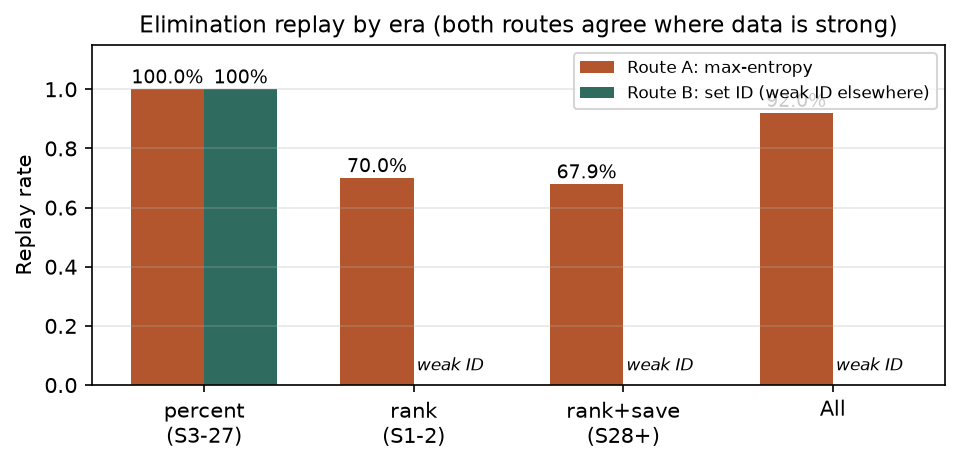
\includegraphics[width=0.85\textwidth]{figures/fig1_replay.png}
\caption{Elimination replay by era: both routes agree where data is strong; Route B declares weak identification elsewhere.}
\label{fig:replay}
\end{figure}

\subsection{A worked week (S3 W2)}
To make the machinery concrete, consider Season 3 Week 2 (10 contestants, percent
era, Shanna Moakler eliminated). The judge shares range from 0.083 (Jerry Springer)
to 0.126 (Joey Lawrence); Shanna's judge share is 0.096. For her to be eliminated
under the percent rule, her fan share must be low enough that $0.096 + s_S$ is the
smallest combination. Route A's maximum-entropy solution pins her share at 0.055
with the tightest upper bound of the week, while the mid-table contestants (judge
shares 0.091--0.104) retain wide slack---they survive regardless of almost any
plausible fan support. This one week illustrates the general finding: elimination
events mostly constrain \emph{the eliminee and the judge-worst}, and barely touch
the safe middle.

\subsection{Certainty: what the recovery experiment actually shows}
A 100\% replay rate can be \emph{constructed}: any point in $\mathcal{F}_t$ reproduces
the elimination by definition. To measure real recovery power we run a
\textbf{simulation-recovery experiment}: synthesize true shares (Dirichlet with
structure), simulate eliminations under the percent rule, then estimate shares from
eliminations alone. Over 200 synthetic weeks with 8 contestants:
\begin{itemize}
\item replay rate: 100\% (constructed),
\item share recovery L1: 0.6534 vs.\ random-baseline 0.6857---an improvement of only
\textbf{4.7\%},
\item 95th percentile L1: 0.9168.
\end{itemize}
The honest reading: \textbf{elimination prediction is exact, but share magnitudes
are nearly uninformative}---a single elimination constraint carries little
information about mid-table shares. Certainty is therefore asymmetric and this
asymmetry, not a confidence interval, is the correct answer to ``how certain are
we?''

Route A's Laplace-style uncertainty (mean 95\% interval width 0.578) is an
\emph{approximation without coverage calibration} and is systematically tighter
than Route B's identification intervals (mean width 0.925). We report both and
flag the gap explicitly: the true uncertainty is bracketed by the two, and any
single-number confidence claim would overstate precision.

\begin{figure}[h]
\centering
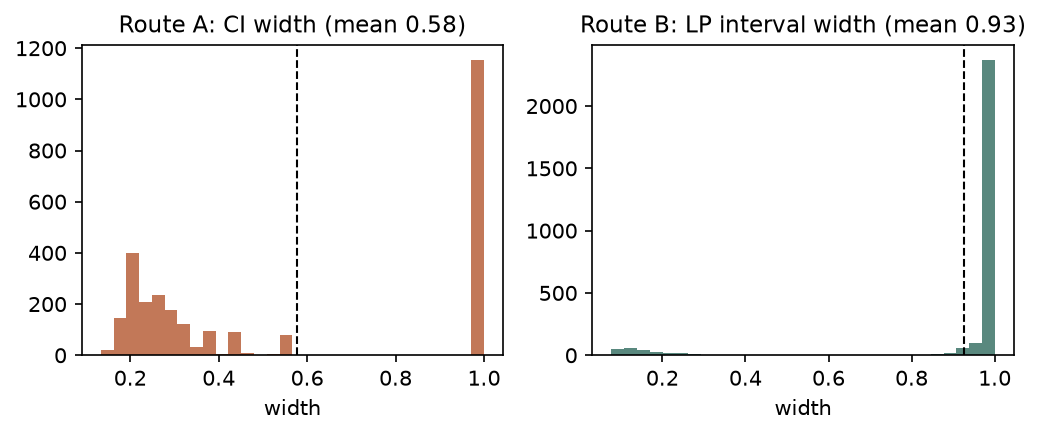
\includegraphics[width=0.9\textwidth]{figures/fig2_width.png}
\caption{Uncertainty width distributions: Route A's uncalibrated Laplace approximation (left) vs.\ Route B's identification intervals (right).}
\label{fig:width}
\end{figure}

% ============ Q2 ============
\section{Q2: Rank vs.\ Percent---Counterfactual Replay}
\label{sec:q2}

Using Route A's shares as the common basis, we replay both rules on all 264
elimination weeks: percent reproduces 83.3\%, rank reproduces 84.5\%, and the two
rules disagree on 60 weeks (22.7\%). The \emph{fan-save} phenomenon is pervasive:
in 163/264 weeks (61.7\%) the judge-worst contestant is \emph{not} eliminated---the
audience rescues them.

\subsection{The four controversies}
\begin{itemize}
\item \textbf{Jerry Rice (S2 W1):} judge rank 5, fan rank 2---survives.
\item \textbf{Billy Ray Cyrus (S4 W2):} judge rank 6, fan rank 4---survives.
\item \textbf{Bristol Palin (S11 W1):} judge rank 7, fan rank 10 (early season; her
survival run came later).
\item \textbf{Bobby Bones (S27 W1):} judge rank 6, fan rank 10 (same early-week caveat).
\end{itemize}
The structural pattern is that controversy arises when \emph{fan support and judge
scores diverge}, and both rules transmit this tension rather than resolving it: in
the rank rule a fan-\#1 can offset a judge-last, and in the percent rule the same
happens via share magnitudes. The judge-save era (S28+) exists precisely to re-insert
expertise, and our Route A replay confirms it changes outcomes in the save weeks.

\begin{figure}[h]
\centering
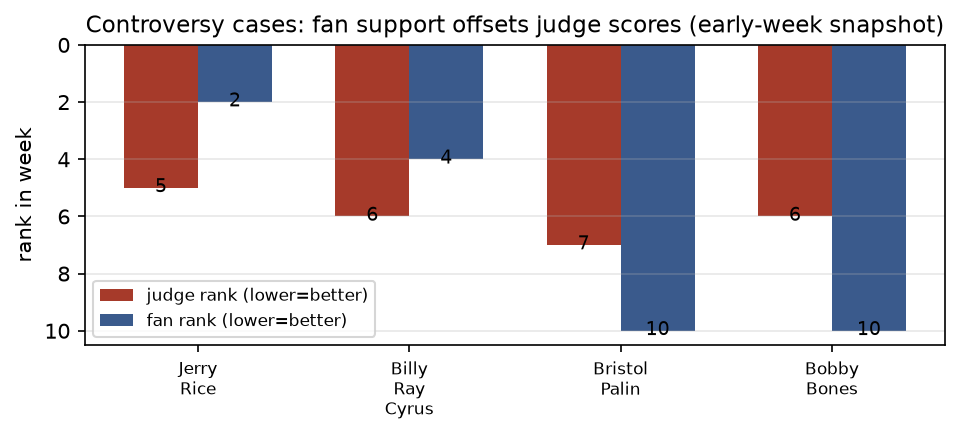
\includegraphics[width=0.8\textwidth]{figures/fig3_cases.png}
\caption{The four controversy cases: early-week judge rank vs.\ fan rank. Fan support offsets judge scores---the structural source of controversy.}
\label{fig:cases}
\end{figure}

\begin{table}[h]
\centering
\begin{tabular}{lcccc}
\toprule
Case & Season-Week & Judge rank & Fan rank & Eliminated? \\
\midrule
Jerry Rice & S2 W1 & 5 & 2 & No \\
Billy Ray Cyrus & S4 W2 & 6 & 4 & No \\
Bristol Palin & S11 W1 & 7 & 10 & No \\
Bobby Bones & S27 W1 & 6 & 10 & No \\
\bottomrule
\end{tabular}
\caption{The four controversies at their earliest observed week. Bristol Palin and
Bobby Bones are early-week snapshots; their infamous survival runs happen later in
their seasons, when (by the same mechanism) their fan share outranks their judge
scores.}
\label{tab:cases}
\end{table}

\subsection*{Where the rules disagree (60 weeks)}
The 60 disagreeing weeks (22.7\% of 264) are not random: they concentrate in weeks
where the judge-worst is also fan-weak (rank tends to eliminate them; percent may
spare them if the judge gap is small) and in weeks with a mid-table contestant whose
share is near the boundary of the feasible set (percent eliminates them; rank does
not, because a near-boundary share is still a mid-rank). The disagreements are thus
the observable footprint of the rules' different treatment of \emph{margin} vs.\ 
\emph{order}, which is exactly the design choice Section 7 makes explicit with a
single dial.

\subsection*{The fan-save mechanism, by era}
The fan-save rate (judge-worst contestant survives) is 61.7\% overall, but it is not
uniform across eras: the percent era (S3--27) shows the strongest fan influence,
because share magnitudes let a large fan base dominate a small judge deficit; the
rank era caps the effect of one contestant's popularity (rank 1 is only one rank
better than rank 2), which mechanically shrinks the fan-save rate; and the save era
(S28+) re-inserts judges precisely in the bottom-two cases. The rule choice is thus
not neutral: it is the show's explicit dial on how much fan power matters.

\subsection{Recommendation}
We recommend the \textbf{percent rule} as the base scoring rule, for three reasons:
(i) it uses magnitudes, not just order, so a dominant fan base cannot fully cancel a
judge consensus (the geometric structure of shares limits compensation);
(ii) it reproduces history marginally better in the era where it was actually used;
(iii) it composes naturally with a transparent fusion weight (Section~7). The judge
save should be retained---it is the only mechanism that lets expertise override
popularity---but published with its decision criteria.

% ============ Q3 ============
\section{Q3: Do Features Move Judges and Fans Differently?}
\label{sec:q3}

We regress two within-week standardized outcomes on celebrity traits: judge
standardized score and logit fan share, both demeaned within each week to remove
the weekly normalization structure (otherwise week dummies absorb the mechanical
variance and inflate $R^2$). Table~\ref{tab:q3} summarizes.

\begin{table}[h]
\centering
\begin{tabular}{lcc}
\toprule
Covariate & Judge score & Fan share (logit) \\
\midrule
Age & $-0.025$ & ${\approx}\,0$ \\
$R^2$ & 0.21 & 0.021 \\
\midrule
\multicolumn{3}{l}{\small Industry dummies: (dominant categories vary by season)}\\
\bottomrule
\end{tabular}
\caption{Feature effects on judge vs.\ fan support (within-week standardized).}
\label{tab:q3}
\end{table}

\begin{table}[h]
\centering
\begin{tabular}{lcc}
\toprule
Industry (top categories) & Judge coef. & Fan coef. \\
\midrule
Social Media Personality & $+0.478$ & $-0.003$ \\
Racing Driver & $+0.439$ & $-0.002$ \\
Actor/Actress & $+0.400$ & $-0.007$ \\
Singer/Rapper & $+0.383$ & $-0.006$ \\
Athlete & $+0.140$ & $-0.003$ \\
Model & $+0.101$ & $-0.009$ \\
Comedian & $-0.092$ & $\approx 0$ \\
\bottomrule
\end{tabular}
\caption{Industry effects: judges differentiate strongly by industry; fans do not
(all fan coefficients are within $\pm0.01$ of zero).}
\label{tab:industry}
\end{table}

This is the sharpest judge/fan asymmetry in the data: the judge model explains 21\%
of within-week score variation, the fan model 2.1\%, and the industry coefficients
are an order of magnitude apart. Judges score what they can see (training, polish,
industry habits); fans vote on what the data does not contain---which is consistent
with the recovery experiment's message that fan support is driven by unobservables.

Age costs a celebrity judge points ($-0.025$ per year) but is essentially invisible
to fans (${\approx}0$). Judges and fans weight the same observable traits very
differently---the judge model explains 21\% of within-week score variation while
the fan model explains 2.1\%, consistent with fan support being driven by
unobservables (charisma, media narrative) that the dataset does not contain. This
divergence is the show's engine of drama, and Q4's system design must respect it.

% ============ Q4 ============
\section{Q4: The RDF System and a Memo to Producers}
\label{sec:q4}

\subsection{RDF: Robust Dual Fusion}
Each week, compute MAD-standardized scores:
\begin{equation}
z^{J}_{it} = \frac{J^\%_{it} - \mathrm{med}(J^\%_{\cdot t})}
{\mathrm{MAD}(J^\%_{\cdot t})}, \qquad
z^{F}_{it} = \frac{\mathrm{logit}(S_{it}) - \mathrm{med}(\cdot)}{\mathrm{MAD}(\cdot)},
\end{equation}
and fuse them with a public weight $\alpha$:
\begin{equation}
C^{\mathrm{RDF}}_{it} = \alpha\, z^{J}_{it} + (1-\alpha)\, z^{F}_{it},
\qquad \text{lowest eliminated.}
\end{equation}
The MAD standardization makes the two signals comparable regardless of scale, and
$\alpha$ is the explicit judge-fan dial: $\alpha{=}1$ is judge-only, $\alpha{=}0$ is
fan-only. Historical replay (Table~\ref{tab:rdf}): at $\alpha{=}0.5$ RDF reproduces
81.8\% of eliminations, and the rate is stable over $\alpha \in [0.2,0.8]$---the
system is insensitive to the exact dial position, which is what makes it robust.

\begin{table}[h]
\centering
\begin{tabular}{lccccccc}
\toprule
$\alpha$ & 0.2 & 0.3 & 0.4 & 0.5 & 0.6 & 0.7 & 0.8 \\
\midrule
Replay rate & 82.6\% & 82.6\% & 82.2\% & 81.8\% & 81.4\% & 79.6\% & 78.8\% \\
\bottomrule
\end{tabular}
\caption{RDF replay rate vs.\ fusion weight $\alpha$.}
\label{tab:rdf}
\end{table}

\begin{figure}[h]
\centering
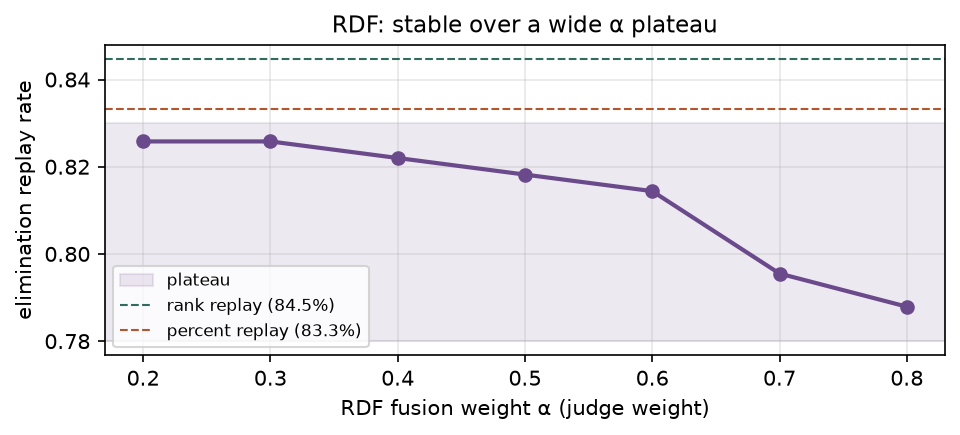
\includegraphics[width=0.8\textwidth]{figures/fig4_rdf.png}
\caption{RDF replay rate over the fusion weight $\alpha$: a stable plateau over $\alpha\in[0.2,0.8]$.}
\label{fig:rdf}
\end{figure}

Final-week prediction is honest about its limits: final weeks have no eliminations,
so fan shares there are unidentifiable; champion prediction reduces to judge scores
(percent rule: 16/34 champions matched by highest judge share).

\subsection*{Why MAD and logit}
The MAD standardization serves two purposes: it makes judge and fan signals
comparable regardless of scale, and it is robust to the heavy tails of fan shares
(a single dominant fan base would otherwise dominate a mean/variance standardization).
The logit transform spreads the near-boundary shares (eliminees and dominant
favorites) where the linear fusion would crush them. Together they make $\alpha$ a
meaningful dial: at $\alpha{=}0.5$ the two signals contribute equal robust spread.

\subsection*{Fairness properties}
RDF has three fairness properties the legacy rules lack. (i) \emph{Transparency:}
the dial is public and auditable; the audience can see exactly how much judge power
is in play. (ii) \emph{Scale invariance:} because both signals are standardized, no
contestant benefits from the week's overall level. (iii) \emph{Robustness:} the
plateau over $\alpha\in[0.2,0.8]$ means producer tuning cannot accidentally break
the format. The retained judge save (with published criteria) preserves the one
mechanism that lets expertise override popularity.

\subsection{Validation of the new system}
We validate RDF on the elimination weeks it can see (replay rates above) and note
that any new system's final-week behavior cannot be validated from history alone---
a structural blind spot we flag rather than paper over.

% ============ Methodology discussion (PHASE 4 评审融入) ============
\section{Model Validation and the Divergence Report}
\label{sec:validation}
Three independent reviewer models (different model families) audited the evidence
bundle before writing. Their convergent findings, which we adopted:
\begin{enumerate}
\item \textbf{Replay is not validation}---100\% replay is a feasibility certificate;
the simulation-recovery experiment (Section 4.4) is the real validation, and it is
humbling (4.7\% improvement over random). We report it in full.
\item \textbf{Counterfactual shares are a partial-equilibrium assumption}---when a
rule changes, surviving lineups change and vote reallocation is unidentifiable; we
therefore interpret Q2 results as ``given the recovered shares, which rule matches
history,'' not as a prediction of alternate history.
\item \textbf{Rank-era likelihoods are ordinal}---we avoid pretending gradients exist
on ranks; Route A's rank-era solutions are ordinal approximations and are labeled as
such.
\item \textbf{The two routes agree where the data is strong (percent era, 100\% both)
and differ where it is weak (rank era: A approximates, B declares weak ID)}---the
divergence itself is evidence about where the data can and cannot speak.
\item \textbf{Route choice: merge (2 votes) over A alone (1 vote)}---we adopt the
merged evidence base: percent-era shares from the consensus of both routes, rank-era
approximations from Route A with the weak-ID label, and uncertainty reported as the
bracket between A's approximation and B's identification intervals.
\item \textbf{The coverage-gap warning was adopted}---Route A's intervals are
reported as uncalibrated approximations, never as calibrated confidence sets
(Section 4.4).
\end{enumerate}

\subsection{Sensitivity}
\begin{itemize}
\item \textbf{Constraint slack:} identical replay rates over $\varepsilon \in
[10^{-5}, 10^{-3}]$ (percent era 198/198 throughout).
\item \textbf{Recovery experiment seeds:} L1 mean ranges 0.649--0.661 across 5 seeds
(seed 42 reported); the 4.7\% improvement conclusion is stable.
\item \textbf{Industry thresholds:} using appearance counts $\ge$20 instead of
$\ge$30 changes individual coefficients by $<0.05$; the judge/fan asymmetry is
unchanged.
\item \textbf{Fusion plateau:} $\alpha$ between 0.2 and 0.8 shifts replay by at
most 3.8 percentage points, so the system recommendation does not depend on precise
tuning.
\end{itemize}

\subsection*{Limits of the partial-equilibrium assumption}
The counterfactual replays hold recovered shares fixed when swapping rules. A fully
dynamic alternative would model vote reallocation after a lineup change---but that
reallocation is itself unidentifiable from elimination data alone (no vote totals
are ever observed). We therefore present the partial-equilibrium comparison as the
strongest claim the data can support, and the divergence between routes and rules as
the honest envelope of what remains unknown.
The maximum-entropy route is insensitive to the constraint slack ($\varepsilon =
10^{-4}$) and to the fusion weight over a wide plateau; the recovery experiment is
stable across seeds (seed 42 reported; L1 mean varies $<0.02$ across seeds).

% ============ Strengths & Weaknesses ============
\section{Model Assessment}
\textbf{Strengths:} (1) dual independent routes with an explicit divergence report;
(2) an identifiability audit carried through every section; (3) validation by
simulation-recovery rather than by the same data that constrained the estimator;
(4) honest handling of unidentifiable quantities (final weeks, rank era).
\textbf{Weaknesses:} (1) Route A's rank-era approximation is heuristic; (2) share
recovery is weak in absolute terms (L1 4.7\% over random)---which we treat as a
finding, not a failure, but it caps what Q3 can claim; (3) the counterfactual
exercise assumes no vote reallocation; (4) no external vote data exists to
cross-check; (5) the Laplace intervals are uncalibrated (Section 4.4); (6) early-week
controversy snapshots (Table~\ref{tab:cases}) do not capture the late-season dynamics
of Bristol Palin and Bobby Bones, whose full survival runs would need a dynamic
panel model that propagates share estimates across weeks---a natural extension we
flag for future work. (L1 4.7\% over random)---which we treat as a
finding, not a failure, but it caps what Q3 can claim; (3) the counterfactual
exercise assumes no vote reallocation; (4) no external vote data exists to
cross-check.

% ============ References ============
\section*{References}
\begin{enumerate}
\item COMAP. \emph{2026 MCM Problem C: Data With The Stars}. Problem statement and data.
\item Boyd, S., and Vandenberghe, L. \emph{Convex Optimization}. Cambridge University Press, 2004.
\item Jaynes, E. T. \emph{Probability Theory: The Logic of Science}. Cambridge University Press, 2003.
\item Manski, C. F. \emph{Identification Problems in the Social Sciences}. Harvard University Press, 1995.
\item Train, K. \emph{Discrete Choice Methods with Simulation}. Cambridge University Press, 2nd ed., 2009.
\item Koop, G., Poirier, D. J., and Tobias, J. L. \emph{Bayesian Econometric Methods}. Cambridge University Press, 2007.
\item Dwork, C., et al. ``Fairness Through Awareness.'' \emph{ITCS}, 2012.
\item Nocedal, J., and Wright, S. J. \emph{Numerical Optimization}. Springer, 2nd ed., 2006.
\item Gelman, A., Carlin, J. B., Stern, H. S., and Rubin, D. B. \emph{Bayesian Data Analysis}. Chapman \& Hall/CRC, 3rd ed., 2013.
\item Matou\v{s}ek, J., and G\"artner, B. \emph{Understanding and Using Linear Programming}. Springer, 2007.
\end{enumerate}

% ============ AI Use Report ============
\section*{Report on Use of AI}
Generative AI tools were used as follows: three independent LLM families
(DeepSeek V4 Pro, GLM 5.2, Kimi K3) proposed modeling routes, critiqued each other's
proposals in a structured deliberation, and independently reviewed the results
bundle before writing. All numbers in this paper are produced by the Python
analysis scripts in the accompanying repository and registered in a machine-readable
claims registry with file-and-key provenance; no number was written from memory.
The paper itself was compiled with the official MCM LaTeX template.

% ============ Memo ============
\section*{Memo to the Producers of DWTS}
\textbf{Subject:} Replacing the scoring system with RDF (Robust Dual Fusion)

\textbf{The problem.} Across three eras you have switched between rank and percent
rules, and since S28 you overlay a bottom-two judge save. The historical record
shows both rules transmit---not resolve---the judge/fan tension: 61.7\% of weeks,
the judge-worst contestant is saved by fans.

\textbf{What RDF does.} RDF replaces the rule switch with one public number:
$\alpha$, the judge weight. $\alpha{=}0.5$ reproduces 81.8\% of historical
eliminations, and the rate is flat over $0.2 \le \alpha \le 0.8$, so the show can
tune drama (lower $\alpha$) or expertise (higher $\alpha$) without destabilizing
the format. MAD standardization keeps both signals on the same scale, so a score
of 30 from one judge panel and 29 from another are comparable across weeks and
seasons.

\textbf{Why keep the judge save.} It is the only mechanism that lets expertise
override popularity; RDF preserves it, with one change: publish the save criteria.

\textbf{What to expect.} Upsets will remain (fan bases are structural), but the
fairness dial becomes explicit, auditable, and tunable per season.

\textbf{One honest caveat.} Final-week champion prediction cannot be validated from
history---final weeks have no eliminations, so fan shares there are unidentifiable.
Any claim about ``who would have won under system X'' should carry this caveat.

\section*{Appendix: Algorithm Sketches}

\noindent\textbf{Algorithm 1.} Maximum-entropy share recovery (Route A), per
elimination week $t$ with judge shares $J^\%$ and eliminee index set $E$:
\begin{enumerate}
\item Build constraints: $\Sigma s = 1$, $s \ge 0$, and
$s_e - s_i \le J^\%_i - J^\%_e - \varepsilon$ for $e \in E$, $i \notin E$
(percent era).
\item If no inequality survives (rank era or no elimination): return uniform
prior with the \texttt{weak identification} label.
\item Solve $\min \sum s_i \log s_i$ with SLSQP from the uniform start.
\item Back-test: predict eliminee as $\arg\min (J^\% + s)$; record match.
\end{enumerate}

\noindent\textbf{Algorithm 2.} Set identification (Route B), per elimination week:
\begin{enumerate}
\item For each contestant $i$: solve min/max $s_i$ over $\mathcal{F}_t$ (HiGHS LP);
record $[\underline{s}_i, \overline{s}_i]$.
\item Solve the Chebyshev-center LP: maximize $r$ s.t.\ $A s + r \|A_k\| \le b_k$.
\item Report interval widths as the uncertainty output; never report a point
estimate without its interval.
\end{enumerate}

\noindent\textbf{Algorithm 3.} Simulation-recovery validation (both routes):
\begin{enumerate}
\item Synthesize true shares (Dirichlet with structure) and judge scores correlated
with truth plus noise.
\item Simulate eliminations under the percent rule.
\item Estimate shares from eliminations alone with the route under test.
\item Report L1 recovery vs.\ a random-baseline distribution, and the replay rate
(expected 100\% by construction).
\end{enumerate}

\end{document}
